\documentclass[12p,a4paper]{article}
\usepackage[utf8]{inputenc}
\usepackage[T1]{fontenc,url}
\usepackage{multicol}
\usepackage{multirow}
\usepackage{parskip}
\usepackage{lmodern}
\usepackage{microtype}
\usepackage{verbatim}
\usepackage{amsmath, amssymb}
\usepackage{tikz}
\usepackage{physics}
\usepackage{mathtools}
\usepackage{algorithm}
\usepackage{algpseudocode}
\usepackage{listings}
\usepackage{enumerate}
\usepackage{graphicx}
\usepackage{float}
\usepackage{hyperref}
\usepackage{tabularx}
\usepackage{siunitx}
\usepackage{fancyvrb}
\usepackage[makeroom]{cancel}
\usepackage[margin=2.4cm]{geometry}
\renewcommand{\baselinestretch}{1}
\renewcommand{\exp}{e^}
\renewcommand{\b}{\boldsymbol}
\newcommand{\h}{\hat}
\newcommand{\m}{\mathbb}
\newcommand{\half}{\frac{1}{2}}
\renewcommand{\exp}{e^}
\renewcommand{\bar}{\overline}
\setlength\parindent{0pt}


\begin{document}
\title{STK1110 -- Oblig 1}
\author{
    \begin{tabular}{r l}
        Jonas Gahr Sturtzel Lunde & (\texttt{jonassl})
    \end{tabular}}
% \date{}    % if commented out, the date is set to the current date

\maketitle

\hspace{10cm}




\section*{Oppgave 1}
\subsection*{a)}
Vi velger oss estimatoren $\hat{\mu} = \bar{X} \approx 276.89$. $90\%$ konfidensintervallet til $\mu$ med $\bar{X}$ estimatoren er utledet i oppgave 2a til å være
\begin{equation}
    P\qty( \bar{X} - t_{0.05,\, n-1}\cdot\frac{S}{\sqrt{n}} < \sigma < \bar{X} + t_{0.95, n-1}\cdot\frac{S}{\sqrt{n}} ) = 0.9
\end{equation}
Setter vi inn for alle verdier, får vi (se vedlagt kode) et $90\%$ konfidensintervall på $[266.4, 287.4]$.


\subsection*{b)}
Vi velger oss estimatoren $\hat{\sigma} = S \approx 26.36$. $90\%$ konfidensintervallet til $\sigma$ med $S$ estimatoren er utladet i oppgave 2b til å være
\begin{equation}
    P\qty(\sqrt{\frac{(n-1)}{\chi_{0.05,\, n-1}}}S < \sigma < \sqrt{\frac{(n-1)}{\chi_{0.95,\, n-1}}}S) = 0.9
\end{equation}
Setter vi inn for alle verdier, får vi (se vedlagt kode) et $90\%$ konfidensintervall på $[20.8, 36.5]$.


\subsection*{c)}
Konfidensintervallene ble utledet under antagelsen om at fordelingen er normalfordelt. Vi er avhengige av å vite fordelingen for å kunne utlede et konfidensintervall, og målingene virker å være normalfordelte. I forventningsverdiens tilfelle kan vi også lene oss på sentralgrenseteoremet, men det er få datapunkter, og dette gjelder uansett ikke for standardavviket.



\subsection*{d)}
Ikke-parametrisk bootstrap gir et $90\%$ konfidensintervall på (se vedlagt kode) $[267.2, 287.2]$ for $\mu$ og $[18.3, 32.4]$ for $\sigma$. Vi sitter altså med

\begin{tabular}{c|c|c}
              & $\mu$ & $\sigma$ \\ \hline
    Analytisk & $[266.4, 287.4]$  &  $[20.8, 36.5]$ \\
    Bootstrap & $[267.2, 287.2]$  &  $[18.3, 32.4]$
\end{tabular}

Som vi ser stemmer intervallet for forventningsverdien $\mu$ meget godt overens, mens det er vesentlige forskjeller i intervallet for standardavviket $\sigma$.



\subsection*{e)}
Vi har en nullhypotese $H_0: \mu = 265$, og en alternativ hypotese $H_a = \mu < 265$. Vi har allerede antatt at dataen er normalfordelt, som betyr at $\bar{X}$ skal være t-fordelt. Dersom nullhypotesen holder, skal $\bar{X}$ være t-fordelt rundt $\mu_0$ som
\begin{equation}
    t = \frac{\bar{X} - \mu_0}{S/\sqrt{n}}
\end{equation}
der vi bruker estimatoren $S$ som erstatning for standardavviket $\sigma$. Vi forkaster nullhypotesen dersom denne verdien er mindre enn $-t_{\alpha} = -  1.734$. Vi har at
\begin{equation}
    t = \frac{276.89 - 265}{26.36/\sqrt{19}} = 1.966
\end{equation}
Dette er åpenbart ikke mindre enn $-1.734$, og nullhypotesen holder. Dett er å forvente, ettersom den alternative hypotesen var at $\mu$ skulle være mindre enn en verdi som allerede er en del mindre enn det observerte gjennomsnittet.

Dersom vi gjør en "two-tailed" test, forkaster vi nullhypotesen dersom $t > t_{0.025} = 2.101$ eller $t < -t_{0.025} = -2.101$. Ingen av disse holder, selv om det nå åpenbart er betydelig nærmere, ettersom det oberserverte gjennomsnittet var på den øvre delen av nullhypotesen.


\section*{Oppgave 2}
\subsection*{a)}
Ettersom ligning (1) fra oppgaven er en t-fordeling med $n-1$ frihetsgrader, vet vi at den følger
\begin{equation}
    P\qty(t_{\alpha/2,\, n-1} < \frac{\bar{X} - \mu}{S/\sqrt{n}} < t_{1-\alpha/2,\, n-1}) = 1-\alpha
\end{equation}
der $t_{\alpha/2,\, n-1}$ og $t_{1-\alpha/2,\, n-1}$ er $\alpha/2$ og $1-\alpha/2$ persentilene til en t-fordeling med $n-1$ frihetsgrader. 

Løser vi ulikheten inni parantesen for $\mu$ får vi at
\begin{equation*}
    \bar{X} - t_{\alpha/2,\, n-1}\cdot\frac{S}{\sqrt{n}} < \mu < \bar{X} + t_{1 - \alpha/2, n-1}\cdot\frac{S}{\sqrt{n}}
\end{equation*}
som er $100(1-\alpha)\%$ konfidensintervallet til $\mu$.



\subsection*{b)}
Ettersom ligning (1) fra oppgaven er kjikvadrat-fordelt med $n-1$ frihetsgrader, vet vi at den tilfredsstiller
\begin{equation}
    P\qty(\chi_{\alpha/2,\, n-1} < \frac{(n-1)}{\sigma^2}S^2 < \chi_{\alpha/2,\, n-1}) = 1 - \alpha
\end{equation}
der $\chi_{\alpha/2,\, n-1}$ og $\chi_{1-\alpha/2,\, n-1}$ er $\alpha/2$ og $1-\alpha/2$ persentilene til en kjikvadrat-fordeling med $n-1$ frihetsgrader. 

Løser vi ulikheten inni parantesen for $\sigma$ får vi at
\begin{equation}
    \sqrt{\frac{(n-1)}{\chi_{\alpha/2,\, n-1}}}S < \sigma < \sqrt{\frac{(n-1)}{\chi_{1-\alpha/2,\, n-1}}}S
\end{equation}
som er $100(1-\alpha)\%$ confidensintervallet til $\sigma$.



\subsection*{c) \& d)}
Kode vedlagt i appendiks. Resultatet presenteres i neste oppgave.



\subsection*{e) \& f)}
I figur \ref{fig:1} er det plottet andelen av de genererte $95\%$ konfidensintervallene som treffer de faktiske $\mu$ og $\sigma$ verdiene til normal- og eksponensialfordelingene. Vi ser at andelen stemmer godt overens med den forventede verdien på $0.95$ for både standardavvik og forventningsverdi for normalfordelingen (med noe støy). Dette er forventet, ettersom konfidensintervallet er utledet med hensyn på en normalfordeling.

De målte konfidensintervallene til forventningsverdien til eksponensialfordelingen stemmer ikke overens med forventet verdi for lave sample sizes, men begynner å nærme seg forventede verdier ved $n \approx 60$. Her begynner sentralgrenseteoremet å gjelde, som sier at den målte forventningsverdien til \textit{enhver} fordeling vil være normalfordelt ved store samples.

Konfidensintervallet til standardavviket til forventningsverdien er feil hele veien, ettersom sentralgrenseteoremet bare gjelder forventningsverdier, og konfidensintervallet vårt ikke er tilpasset en eksponensialfordeling.

\begin{figure}
    \centering
    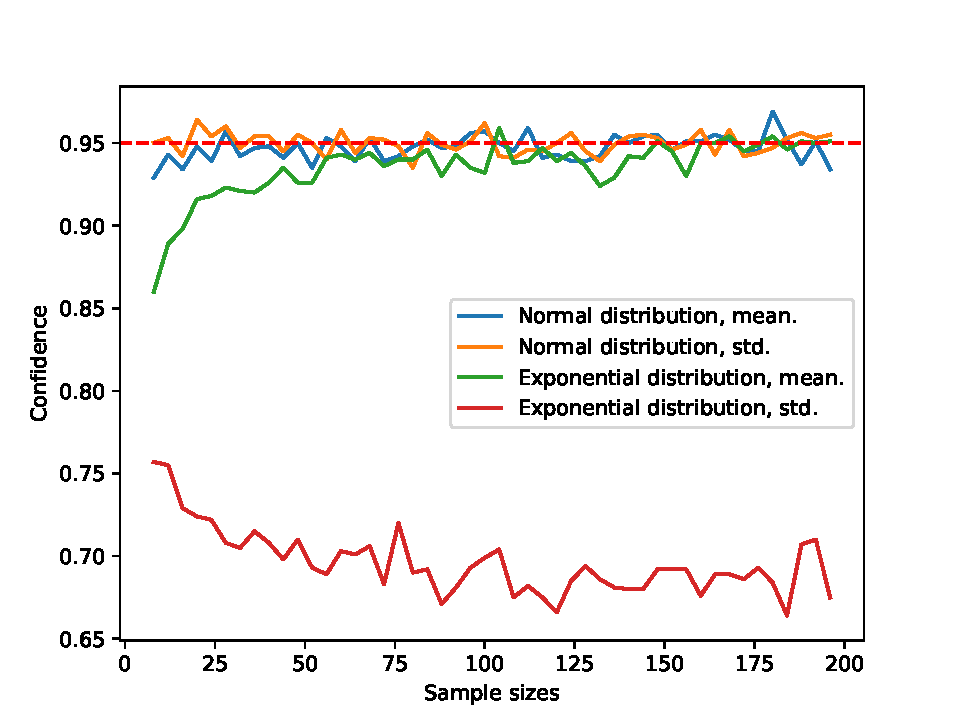
\includegraphics[width=0.7\textwidth]{opg2.pdf}
    \caption{Observerte hit-rates av konfidensintervaller for forventnignsverdi og standardavvik til eksponensialfordeling og normalfordeling mot forventet konfidens.}
    \label{fig:1}
\end{figure}



\section*{Oppgave 3}
\subsection*{a)}
\begin{equation*}
    F(x) = \int\limits_{-\infty}^x f(x) \dd{x} = \int\limits_{\kappa}^x \theta\kappa^\theta x^{-\theta-1} \dd{x} = \qty[\theta\kappa^\theta\frac{x^{-\theta}}{-\theta}]_\kappa^\theta = 1 - \qty(\frac{\kappa}{x})^\theta
\end{equation*}

\begin{equation*}
    F(x) = 1 - \qty(\frac{\kappa}{x})^\theta = \half \ \Rightarrow \ \frac{\kappa}{x} = \frac{1}{2}
\end{equation*}



\subsection*{b)}
\begin{equation*}
    E(X) = \int\limits_{-\infty}^\infty x\cdot f(x) \dd{x}
         = \int\limits_{\kappa}^\infty \theta\kappa^\theta x^{-\theta} \dd{x}
         = \qty[ \theta\kappa^\theta \frac{x^{-\theta+1}}{-\theta+1} ]_{\kappa}^\infty 
         = 0 - \theta\kappa^\theta \frac{\kappa^{-\theta + 1}}{-\theta +1}
         = \frac{\theta\kappa}{\theta - 1}
\end{equation*}



\subsection*{c)}
Vi omskriver den gitte definisjonen til å gi $X$ som definisjon av $Y$:
\begin{align*}
    Y = 2\theta \qty[\ln(X) - \ln(\kappa)] &= 2\theta\ln(X/\kappa) \\
    \exp{Y/2\theta} &= X/\kappa \\
    X &= \kappa \exp{Y/2\theta}
\end{align*}
Vi setter dette inn i uttrykket vårt for den kummulative fordelingsfunksjonen:
\begin{align*}
    F(Y) = 1 - \qty(\frac{\kappa}{\kappa \exp{y/2\theta}})^\theta = 1 - \exp{-y/2}
\end{align*}
\begin{align*}
    f(y) = F'(y) = \half\exp{-y/2} = \frac{1}{2^{2/2}\Gamma(2/2)}x^{2/2-1}\exp{-x/2}
\end{align*}
som vi ser er en kjikvadratfordeling med 2 frihetsgrader.



\subsection*{d)}
\begin{align*}
    E(X) = \frac{\theta\kappa}{\theta - 1} = \bar{X} \ \Rightarrow \ 
    \theta\kappa = \theta\bar{X} - \bar{X} \ \Rightarrow \ 
    \theta = \frac{\bar{X}}{\bar{X} - \kappa}
\end{align*}
Momentestimatoren til $\theta$ er altså $\hat{\theta} = \frac{\bar{X}}{\bar{X} - \kappa}$.



\subsection*{e)}
Sannsynligheten for at kombinasjonen av tilfeldige variable $X_1, X_2,...,X_n$ i $n$ uavhengige forsøk blir $x_1, x_2,...,x_n$ vil være produktet av de individuelle sannsynlighetene
\begin{align*}
    f(x_1, x_2, ..., x_n; \theta) = \prod_{i=1}^n \theta\kappa^\theta\qty(\frac{1}{x_i})^{\theta+1} = \theta^n\kappa^n\theta \qty(\prod_{i=1}^n (x_i)^{-1})^{\theta+1}
\end{align*}

Vi skal finne maks-verdien til denne fordelingen. Vi tar først logaritmen av fordelingen, ettersom den deler toppunkt med sin logaritme, og dette er enklere å regne med.
\begin{align*}
    \ln[f(x_1, x_2, ..., x_n; \theta)]
    &= \ln(\theta^n) + \ln(\kappa^n\theta) + \ln\qty[\qty(\prod_{i=1}^n x_i^{-1})^{\theta+1}] \\
    &= n\ln(\theta) + n\theta\ln(\kappa) + (\theta + 1)\qty[ \sum_{i=1}^n -\ln(x_i) ]
\end{align*}
Deriverer, setter lik 0, og løser for $\theta$:
\begin{align*}
    \dv{\theta} \ln[f(x_1, x_2, ..., x_n; \theta)] &= \frac{n}{\theta} + n\ln(\kappa) - \sum_{i=1}^n \ln(x_i) = 0 \\
    n &= \theta\qty[\sum_{i=1}^n \ln(x_i) - n\ln(\kappa)] \\
    \hat{\theta} &= \frac{n}{\sum_{i=1}^n \ln(x_i) - n\ln(\kappa)}
\end{align*}
som da er maximum likelihood estimatoren for $\theta$.



\subsection*{f)}
Vi har en ny stokastisk variabel
\begin{align*}
    Y = 2n\frac{\theta}{\hat{\theta}} = 2\theta\qty[\sum_{i=1}^n \ln(x_i) - n\ln(\kappa)] = \sum_{i=1}^n 2\theta\qty[\ln(x_i) - \ln(\kappa)] = \sum_{i=1}^n Z
\end{align*}
hvor $Z \sim \chi_2^2$, altså $Z$ er kjikvadratfordelt med 2 frihetsgrader.

Fra s.316 i læreboka har vi at summen av kjikvadratfordelinger selv er en kjikvadratfordeling, med ny frihetsgrad lik summen av frihetsgradene, som betyr at $Z$ er en kjikvadratfordeling med $2n$ frihetsgrader:
\begin{align*}
    \sum_{i=1}^n Z \sim \chi_{2n}^2
\end{align*}



\subsection*{g)}
\begin{align*}
    E[\hat{\theta}] = 2n\theta \cdot E[Y^{-1}]
\end{align*}
Ettersom $Y$ er en kjikvadratfordelt tilfeldig variabel med $\nu = 2n$ frihetsgrader, setter vi inn for dens forventningsverdi, definert i ligning (5) i oppgaven
\begin{align*}
    E[\hat{\theta}] = 2n\theta \cdot \frac{2^{-1} \Gamma\qty(\frac{2n}{2} - 1)}{\Gamma\qty(\frac{2n}{2})} = n\theta\frac{\Gamma\qty(n - 1)}{\Gamma\qty(n)} = n\theta \frac{(n-2)!}{(n-1)!} = \theta\frac{n}{n-1}
\end{align*}

For å finne variansen finner vi først $E[\hat{\theta}^2]$.
\begin{align*}
    E[\hat{\theta}^2] = 2^2n^2\theta^2\cdot \frac{2^{-2} \Gamma\qty(\frac{2n}{2} - 2)}{\Gamma\qty(\frac{2n}{2})} = n^2\theta^2\frac{\Gamma\qty(n - 2)}{\Gamma\qty(n)} = n\theta \frac{(n-3)!}{(n-1)!} = \theta^2\frac{n^2}{(n-1)(n-2)}
\end{align*}

Vi bruker da definisjonen
\begin{align*}
    V[\hat{\theta}] &= E[\hat{\theta}^2] - E[\hat{\theta}]^2
    = \theta^2\frac{n^2}{(n-1)(n-2)} - \theta^2\frac{n^2}{(n-1)^2} \\
    &= \theta^2\frac{n^2(n-1) - n^2(n-2)}{(n-1)^2(n-2)} = \theta^2\frac{n^2}{(n-1)^2(n-2)}
\end{align*}



\subsection*{h)}
Estimatoren er ikke unbiased, fordi forventningsverdien ikke er $\theta$. Biasen til estimatoren er definert som
\begin{align*}
    Bias(\hat{\theta}) = E[\hat{\theta}] - \theta = \frac{1}{n-1}\theta
\end{align*}
Vi ser at vi kan gjøre estimatoren unbiased ved å gange den med $n-1/n$:
\begin{align*}
    \frac{n-1}{n}\hat{\theta} = \frac{n-1}{\sum_{i=1}^n\ln(X_i) - n\ln(\kappa)}
\end{align*}




\newpage
\appendix
\section*{Appendiks}
\subsection*{Kode til oppgave 1}
\lstinputlisting[language=Python, frame=single, basicstyle=\footnotesize]{opg1.py}
\subsection*{Kode til oppgave 2}
\lstinputlisting[language=Python, frame=single, basicstyle=\footnotesize]{opg2.py}

\end{document}
